\subsection{Process view}

In Slice of Pie, concurrency is handled in the controller.

To handle concurrent calls to the controller and to keep user interfaces from blocking when methods
are being called, we have implemented a pattern called the Asynchronous Programming Model (APM; see
Section \ref{sec:APM}).

APM allows for asynchronous calls by allowing a callback to fire when a call finishes. This means that
a client can change from using a method to using its counterparts prefixed with \emph{Begin} and
\emph{End} to opt in for an asynchronous call. This is particularly useful in desktop clients, which
would usually lock up (become unresponsive) while waiting for the longer blocking calls to conclude.

\begin{figure}[htb]
	\centering
	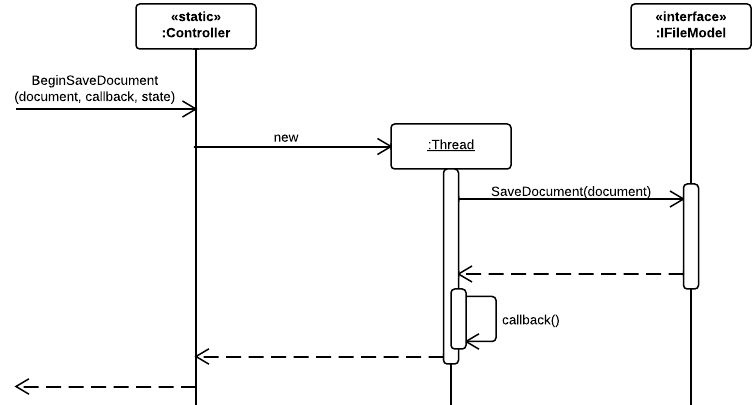
\includegraphics[width=1\textwidth]{Software_architecture/graphics/apm-sequence.png}
	\caption{Sequence Diagram showing the inner workings of any APM call. Instead of using a new Thread, our implementation
        delegates calls to the Thread Pool, to optimize performance (reducing overhead of creating new threads).}
	\label{fig:apm-sequence}
\end{figure}
